\chapter{Introducción}

El drone es un vehículo aéreo no tripulado al que podemos ubicar dentro de la robótica aérea. El proyecto que explica esta memoria se encuadra dentro del manejo, control y recogida de datos de sensores y actuadores de un drone a distancia y su manejo en tiempo real desde un navegador web en un ordenador, tableta o teléfono.\\

En estos últimos años el desarrollo de vehículos aéreos no tripulados ha tenido un avance significativo, sobre todo en aplicaciones de uso civil. Uno de los campos en los que más ha despuntado es en el uso para la grabación de cualquier tipo de eventos, tanto a nivel profesional como a nivel \emph{amateur}.\\

Las tecnologías web son otro campo que ha experimentado un avance enorme en los últimos años, permitiendo crear aplicaciones más complejas y elaboradas. A la vez de ser más potentes se pueden implementar directamente en un navegador, sin necesidad de ningún tipo de instalación en el ordenador del cliente.\\

El fondo del proyecto consiste aunar estos dos campos. Se pretende desarrollar una aplicación web con tecnologías de última generación que permita teleoperar el drone desde un ordenador o dispositivo móvil.\\

En las siguientes páginas se darán unas pinceladas sobre la robótica y su uso actual. También hablaremos sobre los sistemas actuales de control y manejo de drones. Para finalizar daremos una visión global sobre las tecnologías existentes dentro de las comunicaciones en tiempo real (RTC, Real Time Communications), que se pueden emplear para comunicar, por ejemplo, un drone con una estación en tierra.\\

\section{Robótica aérea}

Robótica es la rama de la ingeniería mecánica, ingeniería eléctrica, ingeniería electrónica y ciencia de la computación que se ocupa del diseño, construcción, operación, disposición estructural, manufactura y aplicación de los robots. Estos robots están diseñados para realizar tareas o trabajos que los humanos no podemos, por lo que requieren de cierta inteligencia. Las ciencias y tecnologías de las que depende son, entre otras: el álgebra, los autómatas programables, las máquinas de estados, la mecánica o la informática.\\

Es una rama que ha conseguido grandes avances no sólo en tareas que realizaban con anterioridad personas, sino además en otras que suponen una gran dificultad para ser realizadas por estas ya sea por su complejidad, como ensamblar elementos milimétricos en placas bases, o por realizarse en entornos peligrosos. Por otro lado también se han desarrollado robots domésticos para hacer nuestro día a día más sencillo.\\

Los robots tienen una parte \emph{hardware} y otro \emph{software}. Entre los componentes \emph{hardware} que componen un robot se encuentran: a) las fuentes de alimentación, para dotar de autonomía a los robots; b) sensores, que se asemejan a los órganos sensoriales humanos y que sirven para obtener información del entorno que les rodea como temperatura u objetos próximos; c) actuadores interactuar con el entorno; d) memoria, microprocesadores y e) dispositivos de comunicación, que es la electrónica que se comunica con el dispositivo remoto y permite gobernar los movimientos.\\

Por otro lado el software, es quien da la inteligencia al robot para llevar a cabo las funciones para las que fue diseñado.\\


Dentro de la robótica, la rama de la robótica aérea lleva experimentando desde hace varios años un auge espectacular. A este tipo de robots se les conoce también como Vehículos Aéreo No Tripulados ó UAV (\emph{Unmanned Aerial Vehicle}), y de una manera mas coloquial también como \emph{drones}. Se trata de aeronaves con capacidad de volar sin la presencia de un piloto a bordo que lo controle. Algunos de estos drones tienen la capacidad de volar de manera autónoma, aunque lo más común es que haya un piloto u operador teleoperándolo desde tierra.\\

\subsection{Clasificación y usos de los UAV en general}

Podemos encontrar varios tipos de drones atendiendo a su forma y componentes materiales. Los UAV de ala fija son similares a pequeños aviones y despegan y aterrizan del mismo modo. Estos son capaces de alcanzar altas velocidades. Un ejemplo es el UAV MAVinci. Otro tipo es el de fuselaje sustentador, el cual carece de alas y se sirve del propio cuerpo para producir la fuerza de sustentación que le permite volar. Los de ala rotatoria se asemejan a los helicópteros. Suelen tener cuatro o más motores (cuadricópteros, octocópteros, etc). Tienen la ventaja de poder permanecer cernidos en un punto fijo. Ejemplos de cuadricópteros son el Phantom 4 de DJI y el ArDrone 2.0 de Parrot.\\

En la actualidad los UAV tienen utilidad en múltiples campos. Algunos de ellos son los siguientes:

\begin{itemize}
 \item \textbf{Militares.} Blancos móviles aéreos, reconocimiento de terreno y combate, entre otras tareas. 
 \item \textbf{Vigilancia.} Seguridad en hogares, vigilancia de autopistas, costas, etc. 
 \item \textbf{Inspección y reparaciones.} Fotografiar torres eléctricas, oleoductos, presas, gaseoductos, molinos eólicos, puentes, plataformas petrolíferas, etc, con el objetivo de vigilar o buscar daños que deban repararse.
 \item \textbf{Filmación.} Grabación de vídeo para retransmisiones deportivas, anuncios o escenas de cine difíciles de grabar con cámaras convencionales.
 \item \textbf{Sondas de investigación.} Es posible enviar UAV para obtener datos a partir de sus sensores o tomar muestras de partículas, microorganismos, etc. Por ejemplo, se han realizado estudios de huracanes por medio de medidas de presión y temperatura tomadas por UAV enviados al huracán.
 \item \textbf{Rescates.} Es eficiente para rescatar personas que hayan sufrido accidentes en el mar, montañas, u otras zonas de difícil acceso, o bien víctimas de desastres naturales, contar con la ayuda de UAV que faciliten la localización de supervivientes.
 \item \textbf{Detección de incendios.} Otra utilidad es la detección de focos de fuego, por ejemplo en incendios forestales. En general son útiles para la conservación de reservas naturales o zonas protegidas.
 \item \textbf{Agricultura de precisión}. A través del uso de UAV conseguimos un estudio de las parcelas agrícolas más detallado y preciso, de manera que pueden aplicarse tratamientos de manera localizada. Permite reducir costes, mejorar la rentabilidad de los cultivos y disminuye el impacto ambiental al poder aplicarse productos agroquímicos directamente y exclusivamente a las zonas afectadas.
\end{itemize}


\subsection{Cuadricópteros}\label{sec:quadrotors}

Un cuadricóptero utiliza los principios básicos de un helicóptero, utilizando cuatro rotores en vez uno. Estos rotores se acoplan a un esqueleto, el cual puede tener forma de 'x' o de '+'. Con la primera configuración tendríamos 2 motores delanteros y dos traseros (derecho e izquierdo), mientras que con la segunda configuración habría uno delantero, uno trasero y uno en cada lado. \\

Un problema que tienen que afrontar los helicópteros de un solo rotor, es que este produce una fuerza de torsión en el sentido de giro, por lo que es necesario otro rotor más pequeño perpendicular al principal para producir otra fuerza de sustentación que se oponga a la torsión y que el helicóptero no esté continuamente dando vueltas en torno a su eje vertical. En el caso de los cuadricópteros, al disponer de varios rotores, la solución a este mismo problema hacer que el giro de las hélices de una misma extremidad sea opuesto al giro de las de la otra extremidad, de forma que las torsiones se anulen.\\

Dirigir y controlar el movimiento del vehículo se consigue variando la velocidad relativa de cada rotor para cambiar el empuje y el par motor de cada uno de ellos.\\

Las hélices de los rotores, al girar, producen una fuerza de empuje hacia arriba llamada sustentación que es la que hace que se eleve el aparato. Esta fuerza es perpendicular a la velocidad del fluido relativa a la hélice y está contenida en el plano definido por la misma velocidad y la normal a la superficie de la hélice. Para que el drone despegue, la suma de fuerzas provocadas por cada rotor debe superar su peso. Una vez en el aire, si la suma de fuerzas es igual al peso, el drone permanecerá en una altitud fija o cernido (\emph{hovering}). Para aterrizar, o desplazarse hacia abajo, es necesario hacer que la fuerza resultante sea algo menor que la del peso.\\


Para provocar un giro en sentido horario será preciso aumentar la potencia en los rotores con el sentido contrario, al mismo tiempo que se reduce proporcionalmente la potencia de los otros dos para que la fuerza de sustentación siga constante, ya que en caso contrario el robot se desplazaría en su eje \emph{z}.\\


El movimiento hacia delante-atrás o hacia la derecha-izquierda se consigue disminuyendo la potencia de los rotores que estén en el lado hacia el cual se deba desplazar y aumentando los del lado contrario en igual proporción si el drone debe permanecer a una altura fija. Es decir, para movernos hacia la derecha habrá que disminuir la potencia de los rotores derechos y aumentar la de los izquierdos, de forma que el drone se incline hacia la derecha y la fuerza de sustentación tenga una componente horizontal no nula.\\

La figura \ref{fig:quadrotor_movements} muestra las configuraciones de las diferentes velocidades de los motores cuándo hay un giro hacia la derecha y cuándo el drone va hacia delante.\\

\begin{figure}[h!]
\centering
  \begin{subfigure}[]{60mm}
    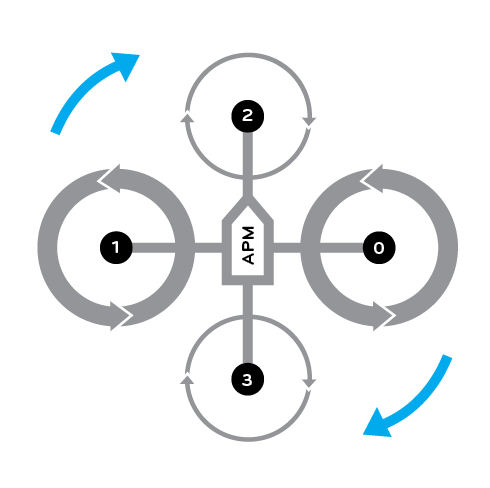
\includegraphics[width=60mm]{quadrotor-rotating}
    \caption{Giro a la derecha.} 
  \end{subfigure}
  \hspace{5pt}
  \begin{subfigure}[]{60mm}
    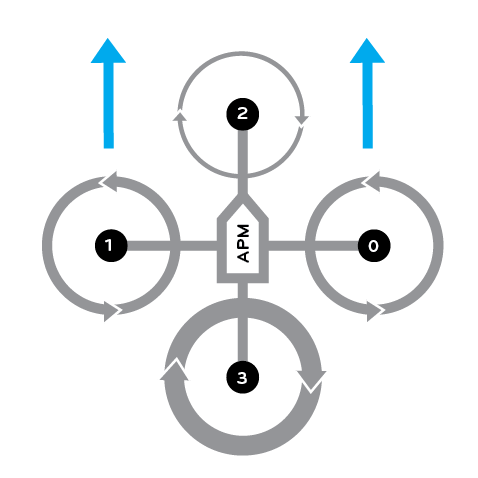
\includegraphics[width=60mm]{quadrotor-forward}
    \caption{Movimiento hacia delante.}
  \end{subfigure}
  \caption{Distintas configuraciones de los motores del cuadricóptero para desplazarse.}\label{fig:quadrotor_movements}
\end{figure}


\subsection{Aplicaciones de los drones}

Debido al auge de los cuadricópteros en los últimos tiempos se han desarrollado proyectos con ellos como elemento principal. Aquí resaltamos algunas de ellas que nos parecen interesantes y representativas.\\

\subsubsection{Lily Drone} 

Lily\footnote{https://www.lily.camera} es un cuadricóptero de reducidas dimensiones y peso (1.3kg) el cuál va equipado con una cámara capaz de grabar vídeo hasta resolución de alta definición a 1080p y 120fps. Lo más llamativo de este drone no son sus capacidades de vuelo ya que sólo nos permite vuelos de hasta 15 metros de altura y unos 40km/h de velocidad, si no que simplemente llevando un dispositivo de detección de reducidas dimensiones (28g), lo enciendes y él, sin necesidad de configuración, lo detecta y sigue todos sus movimientos mientras a la vez te está grabando. Los vuelos son de unos 20 minutos de duración, y el drone es resistente al agua, por lo que puedes usarlo prácticamente en cualquier tipo de situación. Uno de sus puntos fuertes es su funcionamiento en tres pasos, como muestra la figura \ref{fig:lily} (b).\\

\begin{figure}[htb]
\centering
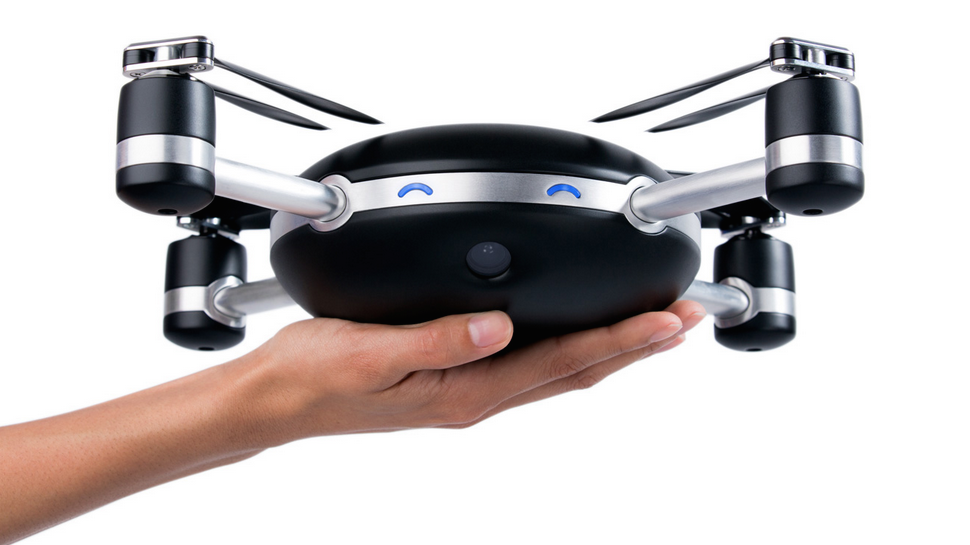
\includegraphics[width=0.7\textwidth]{lily1}
\end{figure}

\begin{figure}[htb]
\centering
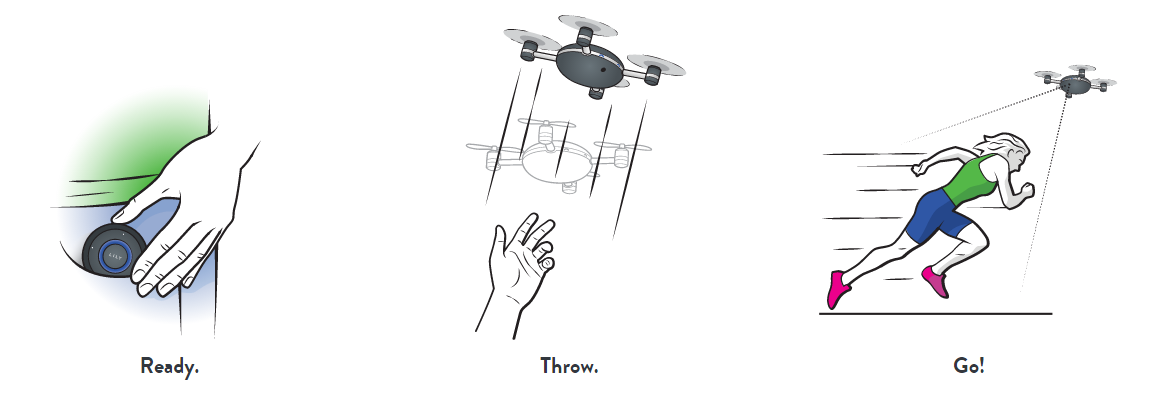
\includegraphics[width=1\textwidth]{lily2}
\caption{Lily (a) y funcionamiento en 3 pasos (b).}
\label{fig:lily}
\end{figure}

\subsubsection{Revisión del tendido eléctrico con drones}

La compañía eléctrica Endesa ha comprado una flota de catorce drones para la revisión de las líneas eléctricas en España. Los drones cuentan con cámara de alta resolución y termográfica. Con el uso de estos aparatos se agilizan las inspecciones, se mejora la calidad y ofrecen mayor seguridad al no tener que trabajar el operario sobre la red. Esto a su vez hace que no sea necesario cortar el suministro eléctrico. La figura \ref{fig:droneendesa} muestra un drone realizando servicios de revisión del tendido eléctrico.\\

\begin{figure}[h!]
\centering
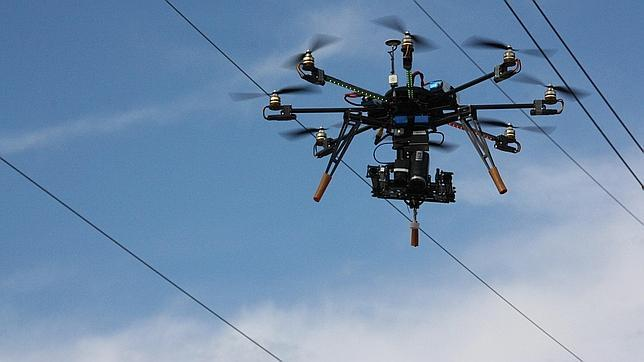
\includegraphics[width=0.8\textwidth]{dronendesa}
\caption{Drone de Endesa realizando labores de revisión.}
\label{fig:droneendesa}
\end{figure}


\subsubsection{Hemav, Agricultura de precisión.}

La empresa Hemav\footnote{http://hemav.com} ofrece entre otros servicios agricultura de precisión a través del vuelos con cuadricópteros. Utilizan sensores multiespectrales y/o térmicos para generar mapas aéreos mediante vuelos autónomos que su suministran información relevante para la toma de decisiones (\ref{fig:hemav} (b)).\\

Posteriormente esa información es analizada estadísticamente para generar patrones de estados, similitudes de terreno, detección de patologías, etc, con los que finalmente se genera un informe con las conclusiones especificas.\\

\begin{figure}[h!]
\centering
  \begin{subfigure}[]{60mm}
    \includegraphics[width=60mm]{hemav2}
    \caption{Hemav.} 
  \end{subfigure}
  \hspace{5pt}
  \begin{subfigure}[]{60mm}
    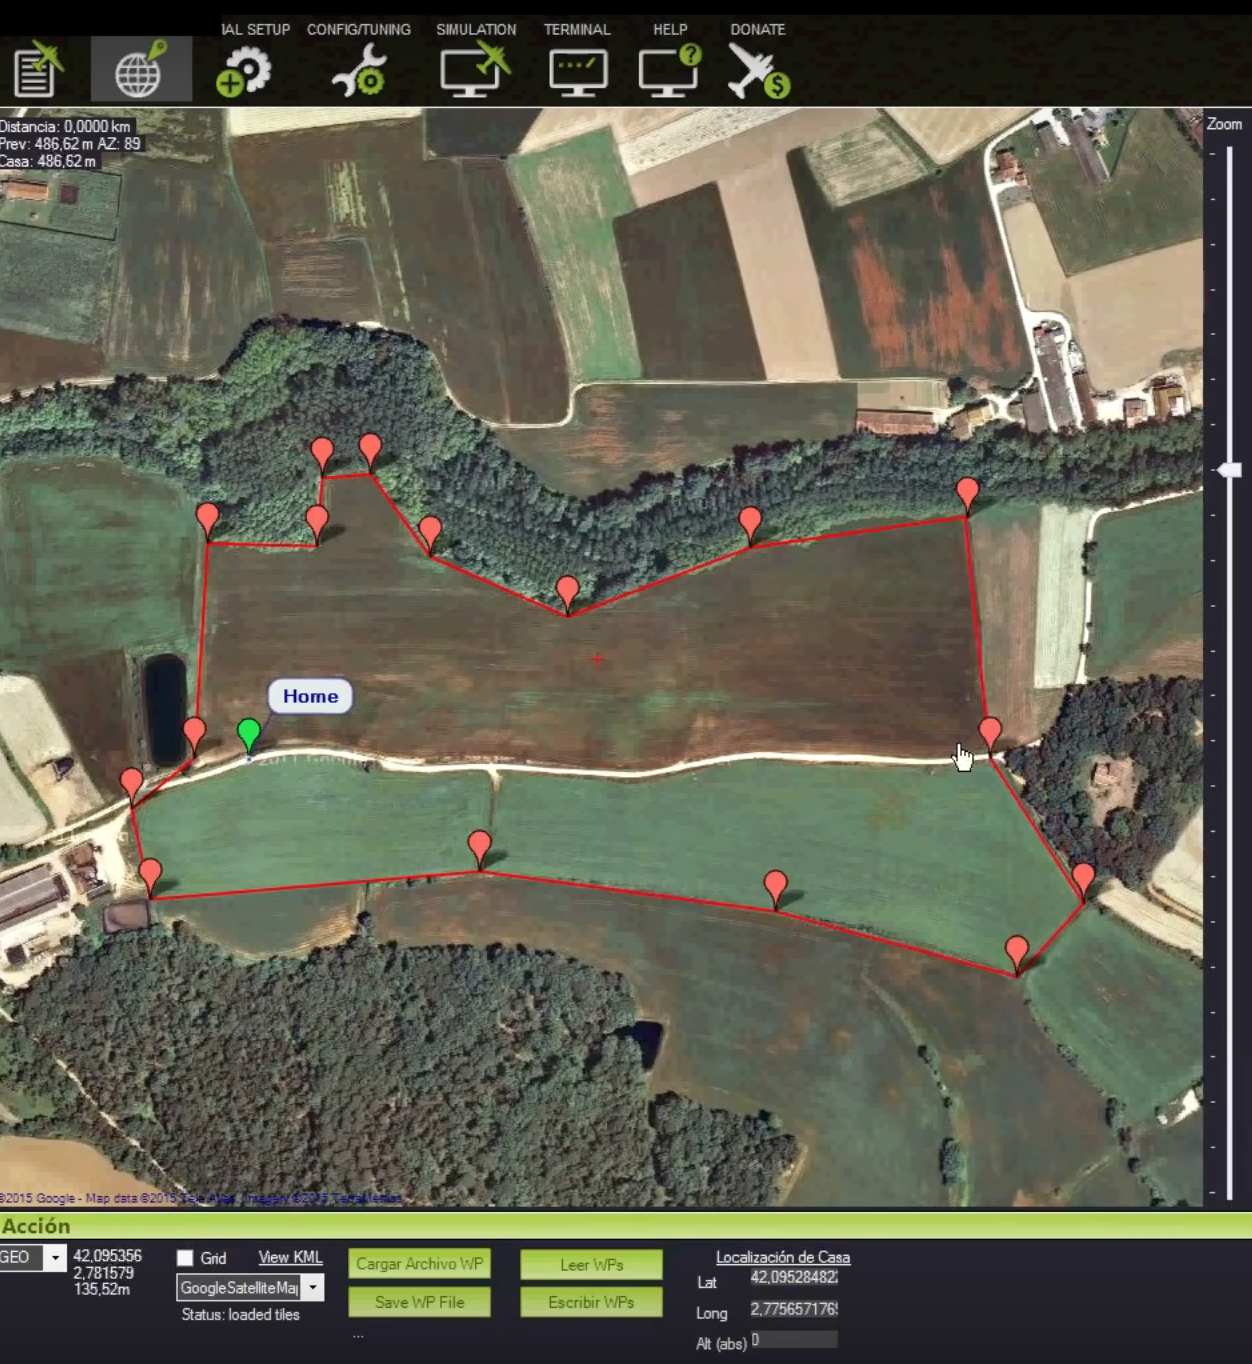
\includegraphics[width=60mm]{hemav1}
    \caption{Finca acotada para el vuelo autónomo.}
  \end{subfigure}
    \caption{Uso de drones en agricultura de precisión.}\label{fig:quadrotor_movements}
  \label{fig:hemav}
\end{figure}


\subsubsection{Entrega de paquetes con drones.}

La entrega de paquetería usando vehículos aéreos no tripulados es el futuro, aunque ya muy presente en prototipos en cuanto a la entrega de paquetes a domicilio se refiere. Las funcionalidades son numerosas, desde entrega de comida o compras realizadas a domicilio, hasta entrega de medicamentos o comida a personas en apuros o situaciones peligrosas.\\

Empresas como Amazon con su proyecto \emph{Prime Air} (figura \ref{fig:amazon}), DHL, Google con \emph{Project Wing} o la NASA están trabajando para desarrollar sus propios sistemas de entrega de paquetería a domicilio a través de drones.\\

\begin{figure}[h!]
\centering
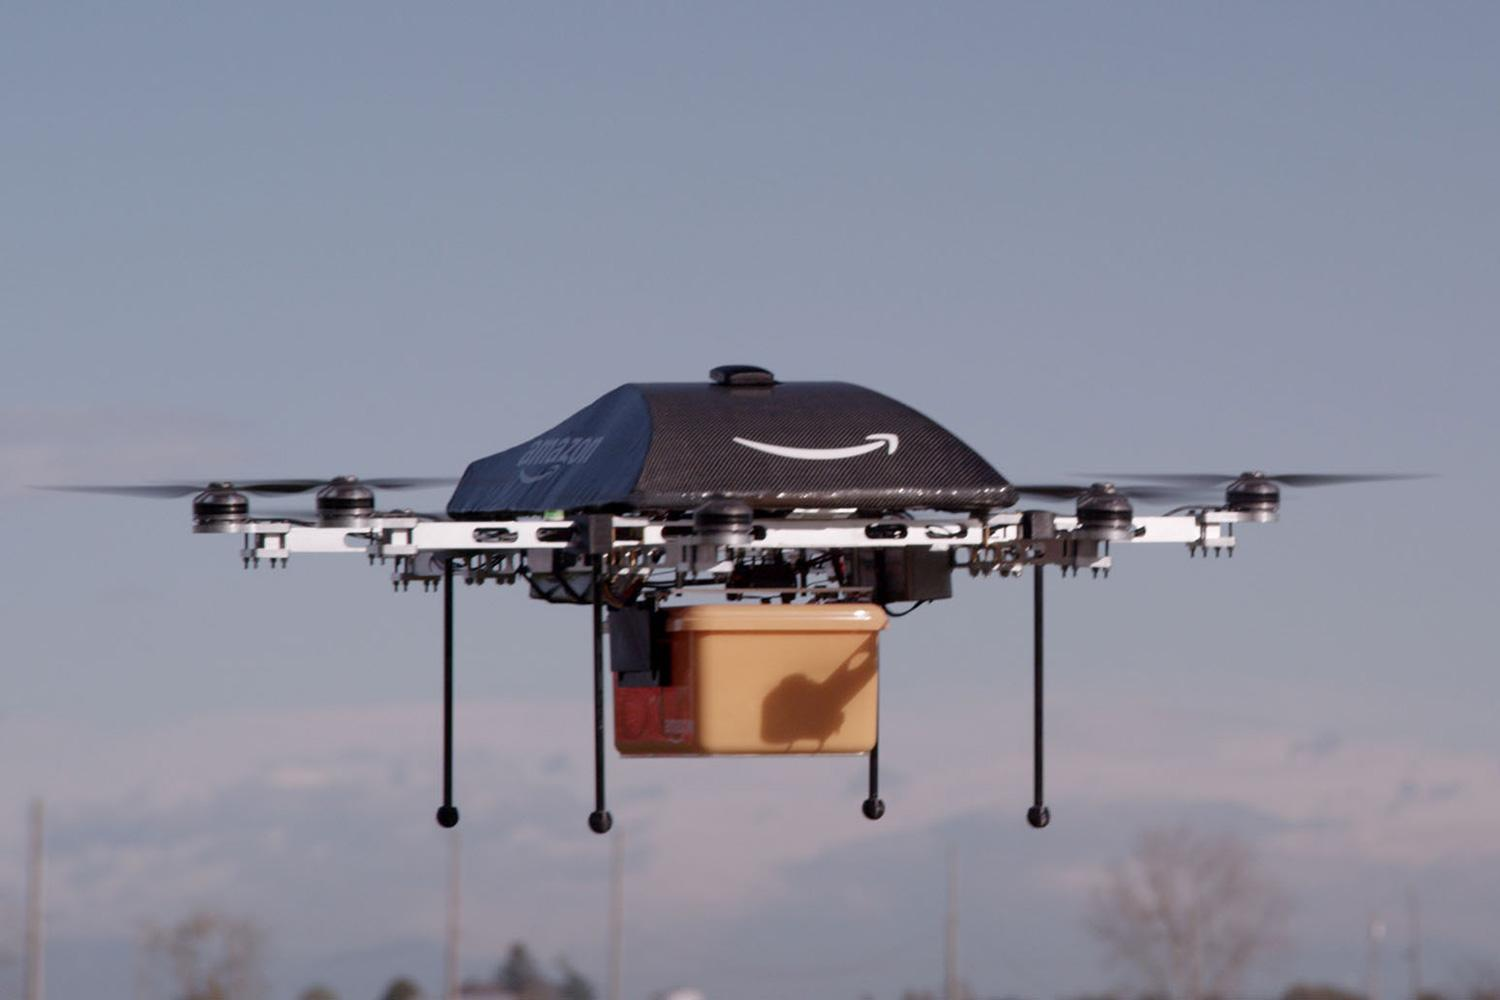
\includegraphics[width=0.9\textwidth]{amazon}
\caption{Amazon Prime Air}
\label{fig:amazon}
\end{figure}

\subsubsection{Drones en salvamento marítimo.}

La Agencia de Medios de Vodafone (MEC) y los expertos de Trabajos con Dron\footnote{trabajoscondrone.com} (TcD) han desarrollado un proyecto de drones socorristas. Estos reducen hasta en tres veces el tiempo en llegar al lugar del accidente con respecto al socorrista tradicional.\\

En caso de incidente, el socorrista-piloto conducirá el drone con el mando de radiocontrol ayudándose de la cámara que lleva a bordo, cuando llega al punto de incidencia lanzara un par de flotadores a los que se pueden agarrar hasta que llegue el equipo de salvamento.\\

En la figura figura \ref{fig:socorrista} se puede ver a un piloto de drones realizando pruebas de salvamento marítimo con un drone.||

 \begin{figure}[h!]
\centering
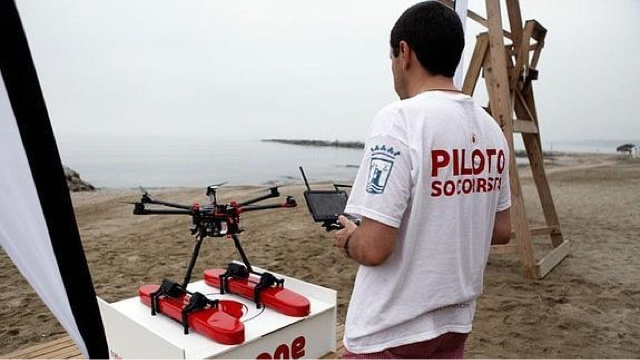
\includegraphics[width=0.9\textwidth]{socorrista}
\caption{Drone de Salvamento Marítimo}
\label{fig:socorrista}
\end{figure}

\subsubsection{Drones en el cine y televisión.}

Hace tiempo que los robots teledirigidos participan en los rodajes, pero sólo recientemente han pasado de tener un papel secundario a convertirse en protagonistas. En la industria cinematográfica se ha añadido el uso del drone para grabar escenas que antes eran complicadas, costosas o imposibles de grabar. Han cobrado tanta importancia que hasta han creado certámenes como el \emph{Flying Robot International Film Festival}\footnote{http://friff.co} para premiar su uso en la grabación. Los drones nos proporcionan nuevas perspectivas en todo tipo de secuencias.\\

Películas como el Lobo de Wall Street, Jurassic World o Skyfall han incorporado entre sus métodos de grabación la utilización de drones. También se utilizan en el mundo de la televisión. Entre otros el famoso programa inglés \emph{Top Gear} o el documental de la BBC Planeta Tierra. En la figura \ref{fig:dronefilm} podemos ver un drone grabando una escena.\\

\begin{figure}[h!]
\centering
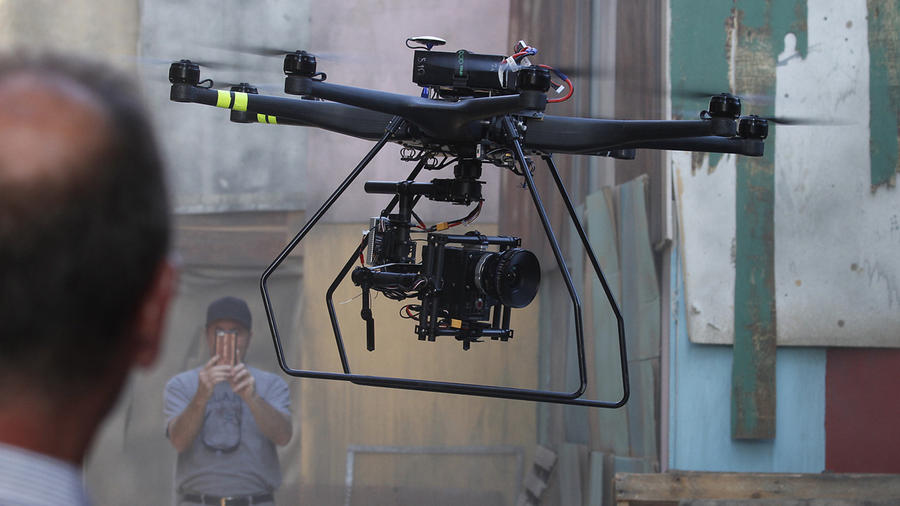
\includegraphics[width=0.9\textwidth]{dronefilm}
\caption{Uso de un drone para grabación.}
\label{fig:dronefilm}
\end{figure}



\subsection{Sistemas de control de drones}
\label{cap:controldrones}

Hay varios sistemas que nos permiten teleoperar o controlar un drone, los cuáles se pueden dividir en dos grupos, los controlados mediante radiofrecuencia y los que usan sistemas alternativos.\\

\emph{\textbf{Radiocontrol:}} Es la técnica que permite el gobierno de un objeto a distancia de manera inalámbrica mediante una emisora de control remoto. Por otra parte, a bordo del vehículo, en nuestro caso un drone, debe ir una receptora de radio control. La comunicación entre receptor y transmisor se efectúa mediante radiofrecuencia, existiendo diferentes sistemas de emisión, como AM, FM o 2.4Ghz con diferentes tipo de codificación, PCM, PPM…\\

Estos sistemas tienen varias limitaciones. Una es el número de canales máximo del sistema, ya que se usa un canal para cada elemento de control disponible: elevación, giro, rotación… La segunda, y posiblemente más crítica, son las interferencias. Si se producen interferencias ya sea por ruido o por varios emisores trabajando en las cercanías se puede perder el control de la aeronave produciendo una posible colisión, destruir la misma o incluso dañar a personas.\\
 

\emph{\textbf{Sistemas alternativos:}} A parte del radiocontrol tenemos el control a través de WiFi. Este sistema consiste en la creación de una red WiFi por parte del drone a la cual se conecta el dispositivo con el que se maneja. Este dispositivo puede ser un mando diseñado y comercializado por la propia marca o un dispositivo móvil, el cuál usa una aplicación que es la que gestiona la conexión y transferencia de datos.\\

La ventaja de estos sistemas es el ahorro de batería, ya que los transmisores y antenas WiFi necesitan de menos potencia para cubrir las mismas distancias que los sistemas tradicionales de radiocontrol. Además, el ancho de banda que nos proporciona es bastante elevado y podremos transferir tanto datos como las imágenes de las cámaras HD a bordo del drone.\\

Empresas como DJI usan sistemas mixtos que consisten en teleoperar el drone vía radiocontrol, pero la gestión y visualización de la cámara se realiza mediante una conexión WiFi como la explicada anteriormente.\\
 
La empresa francesa Parrot, la cual tiene una flota de diversos modelos de drones, utiliza un sistema de red WiFi, a la cuál conectas un dispositivo móvil ya sea Android o iOS, y mediante una aplicación desarrollada por ellos se puede teleoperar el drone, así como tener otras funcionalidades como la grabación de vídeo, captura de imágenes y gestión de parámetros de vuelo como altura o velocidad máxima. En capítulos posteriores profundizaremos en este sistema implementado, ya que es el que usaremos como referencia para desarrollar el nuestro. En la figura \ref{fig:wifiardrone} se muestra cómo se teleopera el cuadricóptero ArDrone 2.0 de Parrot.\\


\begin{figure}[h!]
\centering
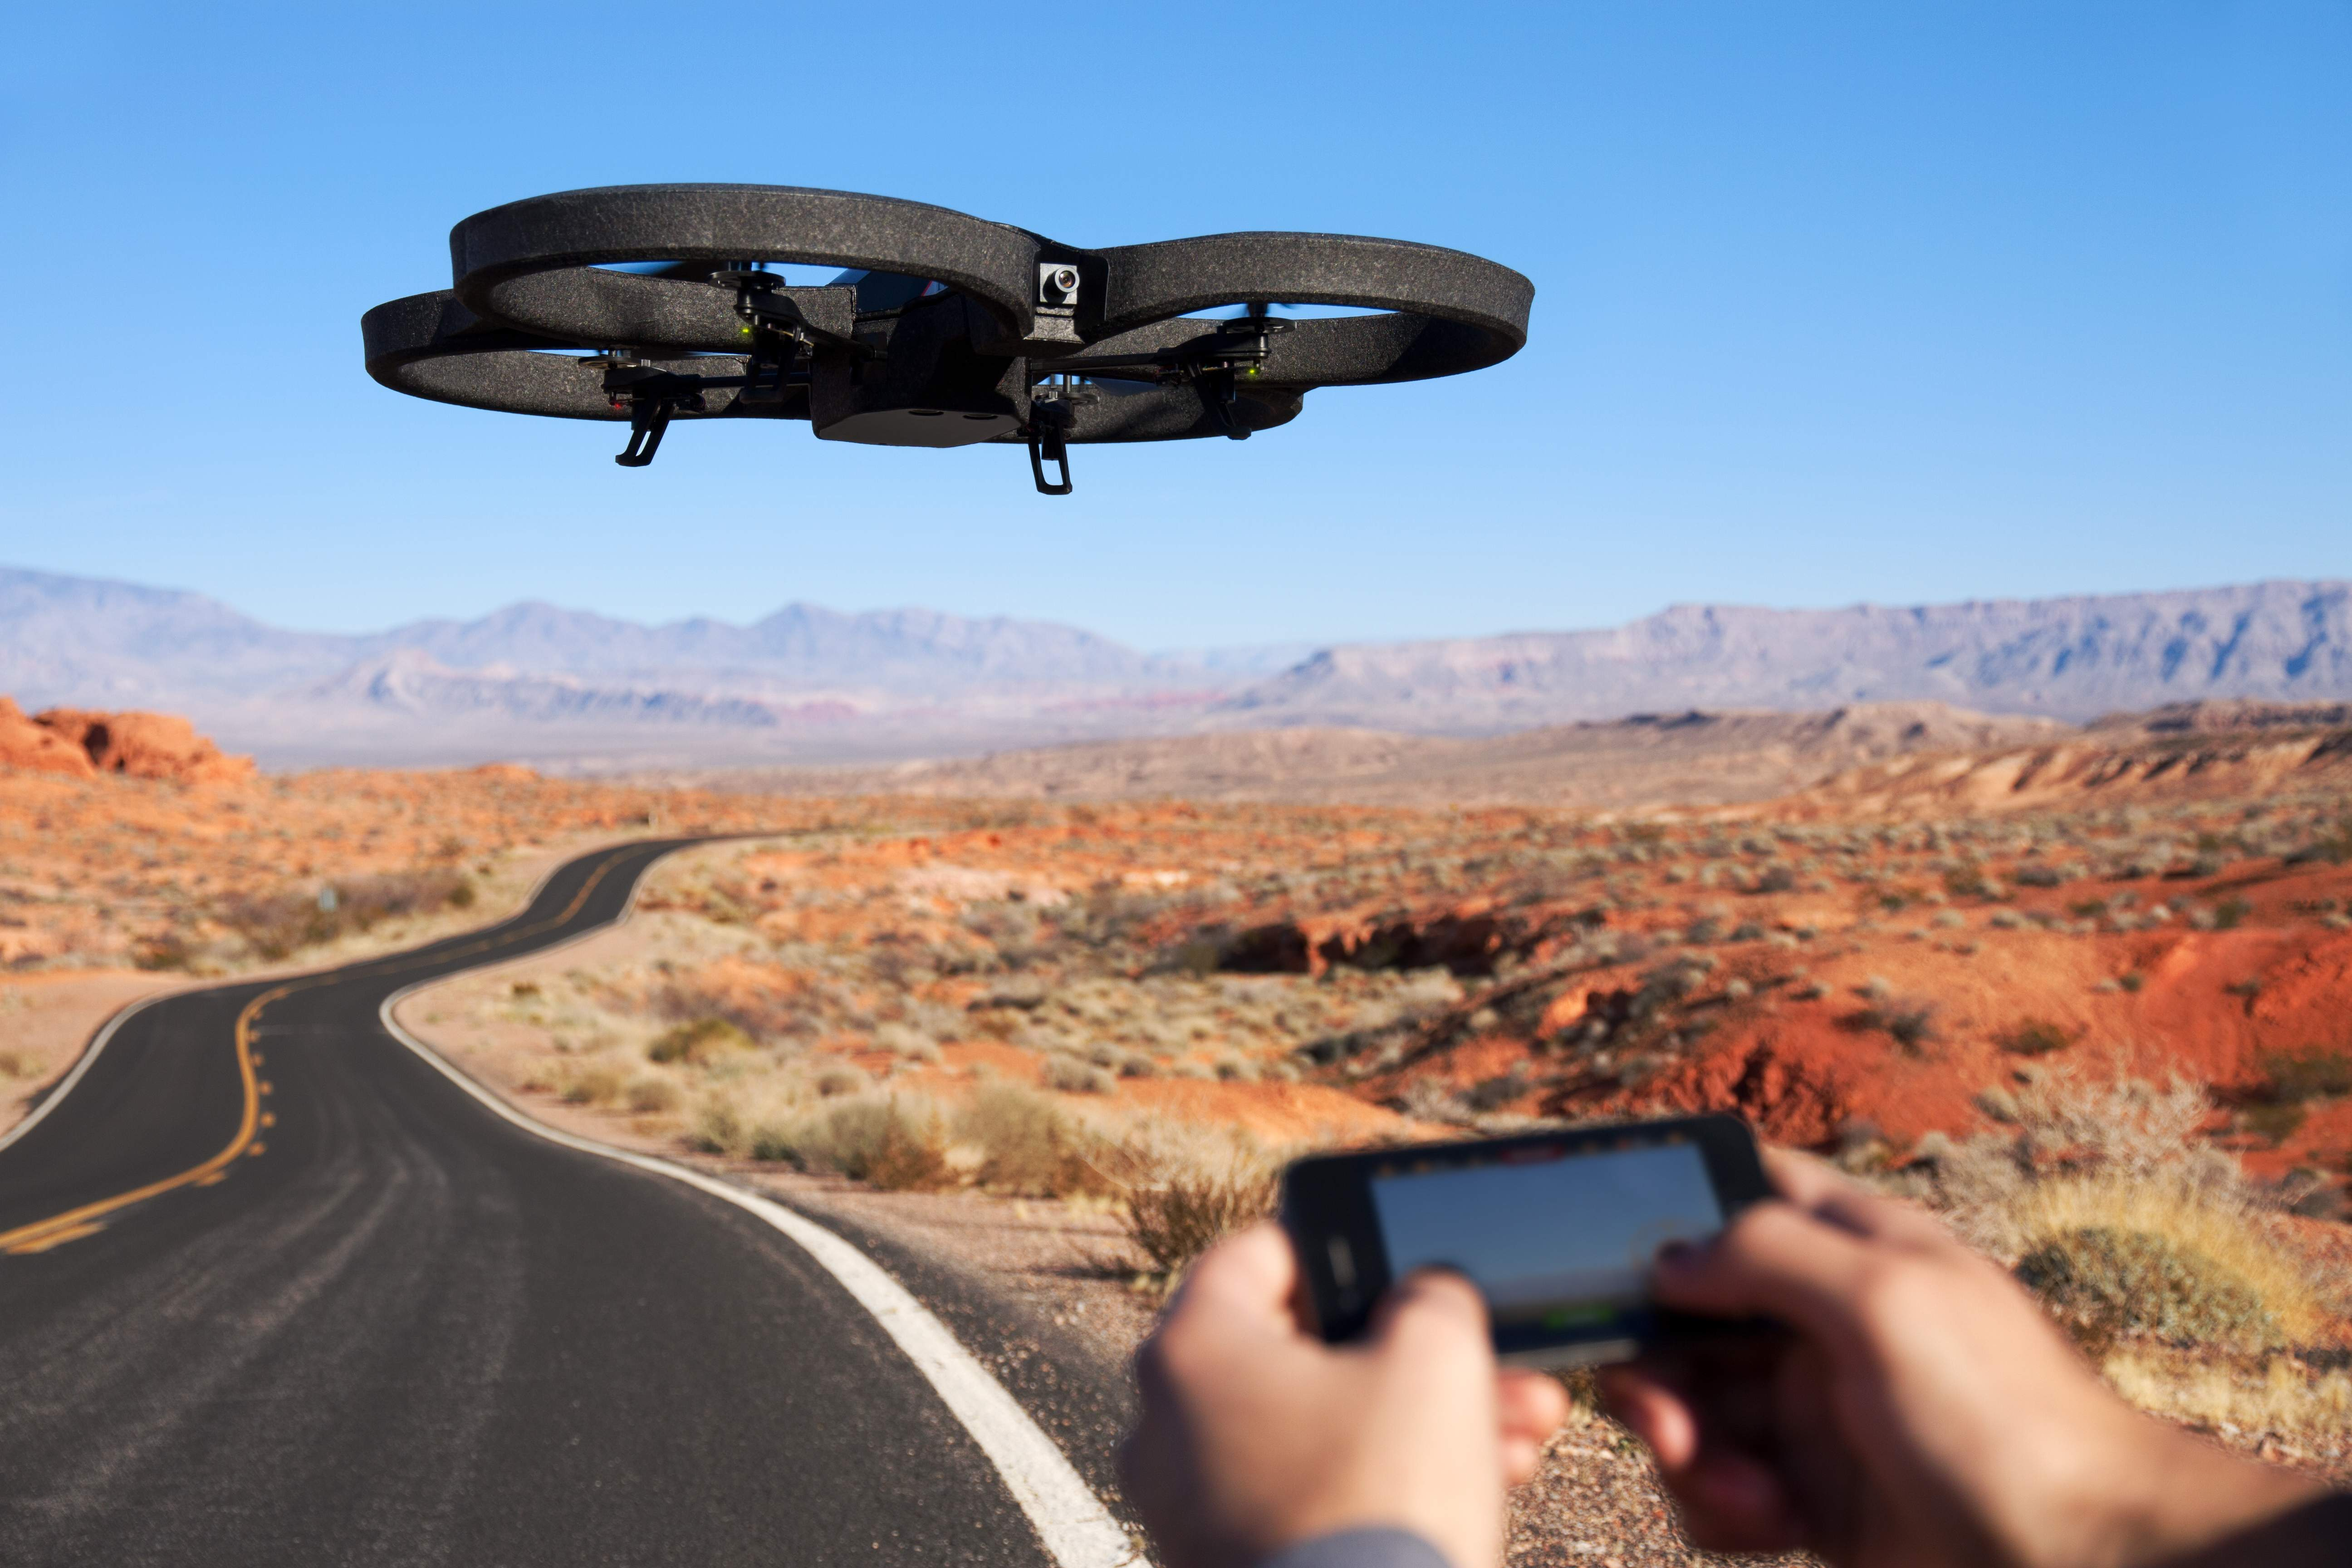
\includegraphics[width=0.8\textwidth]{wifiardrone}
\caption{Sistema WiFi de control del drone de Parrot.}
\label{fig:wifiardrone}
\end{figure}


\section{Tecnologías de comunicación en tiempo real}

En la actualidad  existen numerosas tecnologías de comunicación en tiempo real, pero nos centraremos en las que nos ofrecen conectividad multimedia. Primero veremos protocolos que se pueden implementar en aplicaciones de escritorio, y posteriormente veremos los protocolos web más actuales.\\

\subsection{RTP}

\emph{RTP} son las siglas de \emph{Real-time Transport Protocol} o Protocolo de Transporte en Tiempo Real, el cuál es un protocolo para aplicaciones de escritorio y de nivel de sesión utilizado para la transmisión de información en tiempo real, como por ejemplo audio, vídeo y datos. Está desarrollado por el grupo de trabajo de transporte de audio y vídeo del IETF (\emph{Internet Engineering Task Force}). Este protocolo es la base de la industria de Voz sobre IP (\emph{VoIP}).\\

Se encapsula sobre UDP y usa un puerto de usuario para cada medio que transfiere. Admite direcciones de destino tanto \emph{unicast} como \emph{multicast}. Se encarga de enviar cualquier tipo de trama generada por cualquier algoritmo de codificación como H261, MPEG-1, MPEG-2... pero no añade ningún tipo de fiabilidad ni de calidad del servicio (\emph{QoS}). Lo único que incorpora son marcas de tiempo para evitar el tembleque o \emph{jitter} y la sincronización entre flujos en el destino y números de secuencia para detectar pérdidas en un flujo.\\

RTP trabaja junto con otros dos protocolos que lo complementan. El primero es RTCP (\emph{Real time Control Protocol}), protocolo que proporciona información de control sobre la calidad de la transmisión. Transmite paquetes periódicos asociados a cada flujo RTP que incluye los detalles sobre los participantes, si hubiese más de uno, y las estadísticas de pérdidas que permiten el control de flujo y congestión. Según estas estadísticas se puede hacer codificación adaptativa para adaptarse al medio. También trabaja sobre UDP y usa un número de puerto superior al que usa el flujo de RTP.\\

El segundo es RTSP (\emph{Real Time Streaming Protocol}), protocolo que permite realizar un control remoto de sesión de transmisión multimedia. Es un protocolo independiente del protocolo de transporte, basado en texto que permite recuperar un determinado medio de un servidor o grabar una multiconferencia.\\

La norma define también el protoclo SRTP (\emph{Secure Real-time Transport Protocol}), el cuál es una extensión del perfil de RTP para conferencias de audio y vídeo que puede usarse para proporcionar confidencialidad, autenticación de mensajes y protección de reenvío para flujos de audio y vídeo.\\


\begin{figure}[h!]
\centering
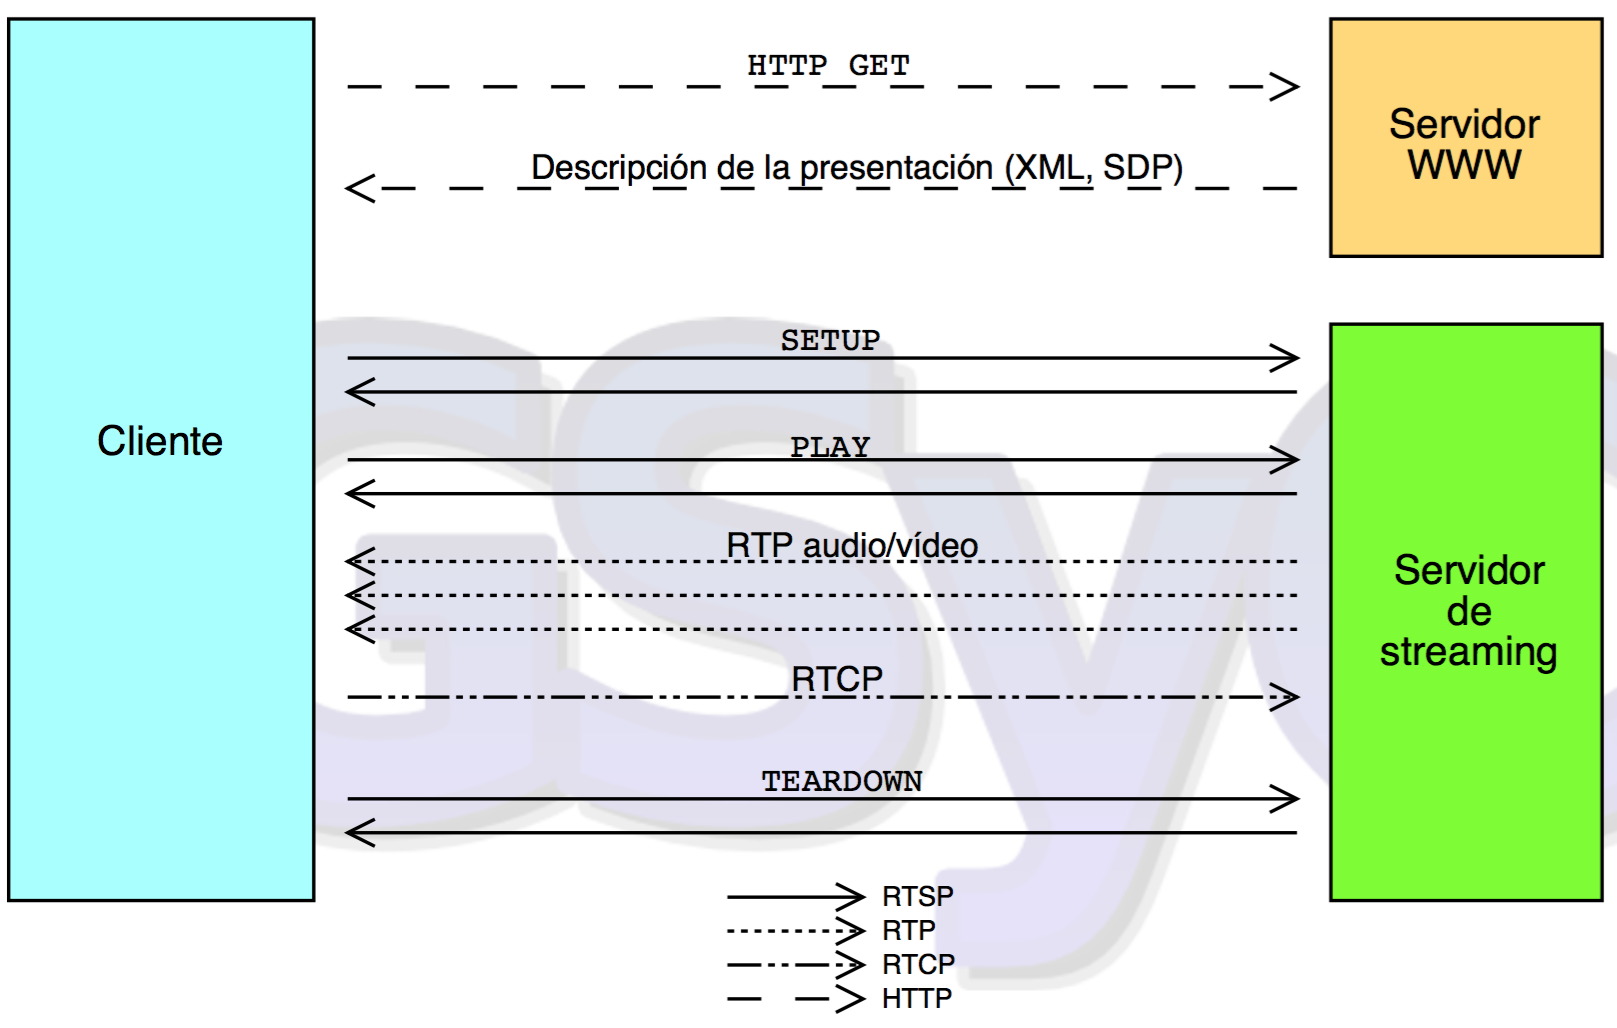
\includegraphics[width=0.8\textwidth]{rtc}
\caption{Ejemplo de conexión RTC, RTCP y RTSP}
\label{fig:rtc}
\end{figure}


\subsection{SIP}

SIP o Protocolo de Inicio de Sesiones (\emph{Session Initiation Protocol}) es un protocolo desarrollado por el grupo de trabajo MMUSIC del IETF con la intención de ser el estándar para la iniciación, modificación y finalización de sesiones interactivas de usuario donde intervienen elementos multimedia como vídeo, voz, mensajería instantánea...\\

Técnicamente no es un protocolo que transmite flujos multimedia, si no que es un protocolo de señalización cuya función es preparar el establecimiento y la terminación de sesiones multimedia entre máquinas remotas. Una de sus más importantes funciones es el intercambio de las descripciones de sesión (\emph{SDP}) de los usuarios. El concepto de sesión en este protocolo es muy amplio: una llamada entre dos, una videoconferencia, un juego interactivo entre varios usuarios...\\

Es un protocolo muy ligero. Tiene solo 6 métodos basados en texto, de manera similar a HTTP o SMTP, pero es completamente independiente del protocolo de transporte utilizado (TCP, UDP, ATM, etc). \\

En la figura \ref{fig:sip} podemos ver un ejemplo de una conexión multimedia con RTP que utiliza el protocolo SIP para establecer y finalizar la sesión entre los dos usuarios.\\

Es el protocolo señalizador para el protocolo RTP explicado anteriormente. Entre otras, Ekiga, WengoPhone, MS Windows Messenger, Apple iChat AV ó Asterisk son algunas aplicaciones que utilizan SIP.\\


\begin{figure}[h!]
\centering
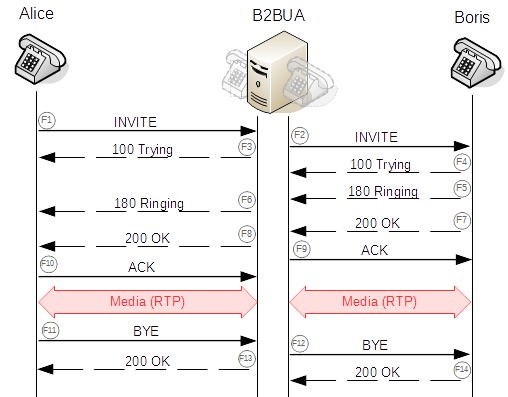
\includegraphics[width=0.8\textwidth]{sip}
\caption{Ejemplo de conexión SIP}
\label{fig:sip}
\end{figure}



\subsection{ORTC}

\emph{Object RTC} es un proyecto de código abierto que permite la comunicación en tiempo real (\emph{RTC, Real-Time Communications}) de dispositivos móviles con servidores u otros navegadores con el simple uso de unas API's JavaScript nativas en el navegador. El objetivo de Object RTC es permitir crear comunicaciones en tiempo real con una alta calidad en dispositivos móviles y servidores con el simple uso de JavaScript y HTML5. Es también una obligación para ORTC ser compatible con WebRTC.\\

Aunque ORTC es un proyecto respaldado por empresas de la talla de Hookflash, Microsoft o Google, por el momento no es una especificación del consorcio W3C (\emph{World Wide Web Consortium}).\\

ORTC comparte muchas similitudes con WebRTC. Como mayor diferencia tenemos que ORTC no utiliza SDP ni el protocolo de Oferta/Respuesta, en cambio utiliza los objetos 'enviador' (\emph{sender}), 'recibidor' (\emph{receiver}) y 'transporte' (\emph{transport}), los cuales tienen capacidades que describen que pueden hacer y sus parámetros que definen como están configurados. Además ORTC no está disponible nada más que en el navegador Edge de Microsoft.\\


\subsection{WebRTC}

En mayo de 2011 Google liberó un proyecto de código abierto basado en la comunicación entre navegadores en tiempo real. El proyecto ha sido continuado estandarizando los protocolos en el IETF y las API's de JavaScript en el W3C. En el consorcio W3C WebRTC es aún un borrador de un proyecto en marcha el cuál está altamente implementado en los navegadores como Mozilla Firefox y Google Chrome. La API está basada en el trabajo previo realizado por \emph{Web Hypertext Application Technology Working Group} (WHATWG).\\

Esta tecnología nos brinda la capacidad de crear numerosas aplicaciones de comunicaciones entre navegadores, sin necesidad de servidores internos, y está llamada a ser el futuro de las comunicaciones en tiempo real.\\


\section{Antecedentes}

Como base para el proyecto tenemos los siguientes trabajos, desarrollados también por alumnos de la URJC. Todos estos proyectos tienen en común que utilizan como base las herramientas que nos ofrece JdeRobot, que es el marco \emph{software} en el que se ubica el presente trabajo.\\

\subsection{ArDroneServer}

ArDroneServer\footnote{\url{http://jderobot.org/Amartinflorido-tfg}}\cite{ArDroneServer} es un \emph{driver} para manejar drones desde la plataforma JdeRobot. Utiliza la SDK de ArDrone de Parrot, ha sido desarrollado por Alberto Martín como parte de su Grado Fin de Carrera. Esta aplicación esta inspirada en los paquetes ROS \emph{ardrone\_brown} y \emph{ardrone\_autonomy}. Implementa tres interfaces que nos permites recibir las imágenes del drone, controlar el drone y recoger información de los sensores y cambiar la configuración del drone. Junto a este servidor Alberto ha desarrollado una aplicación capaz de hacer seguimiento horizontal y vertical de objetos.\\

En la figura \ref{fig:ardroneserveralberto} vemos a Alberto realizando un experimento, en el que el drone hace seguimiento vertical de un objeto.\\

\begin{figure}[h!]
\centering
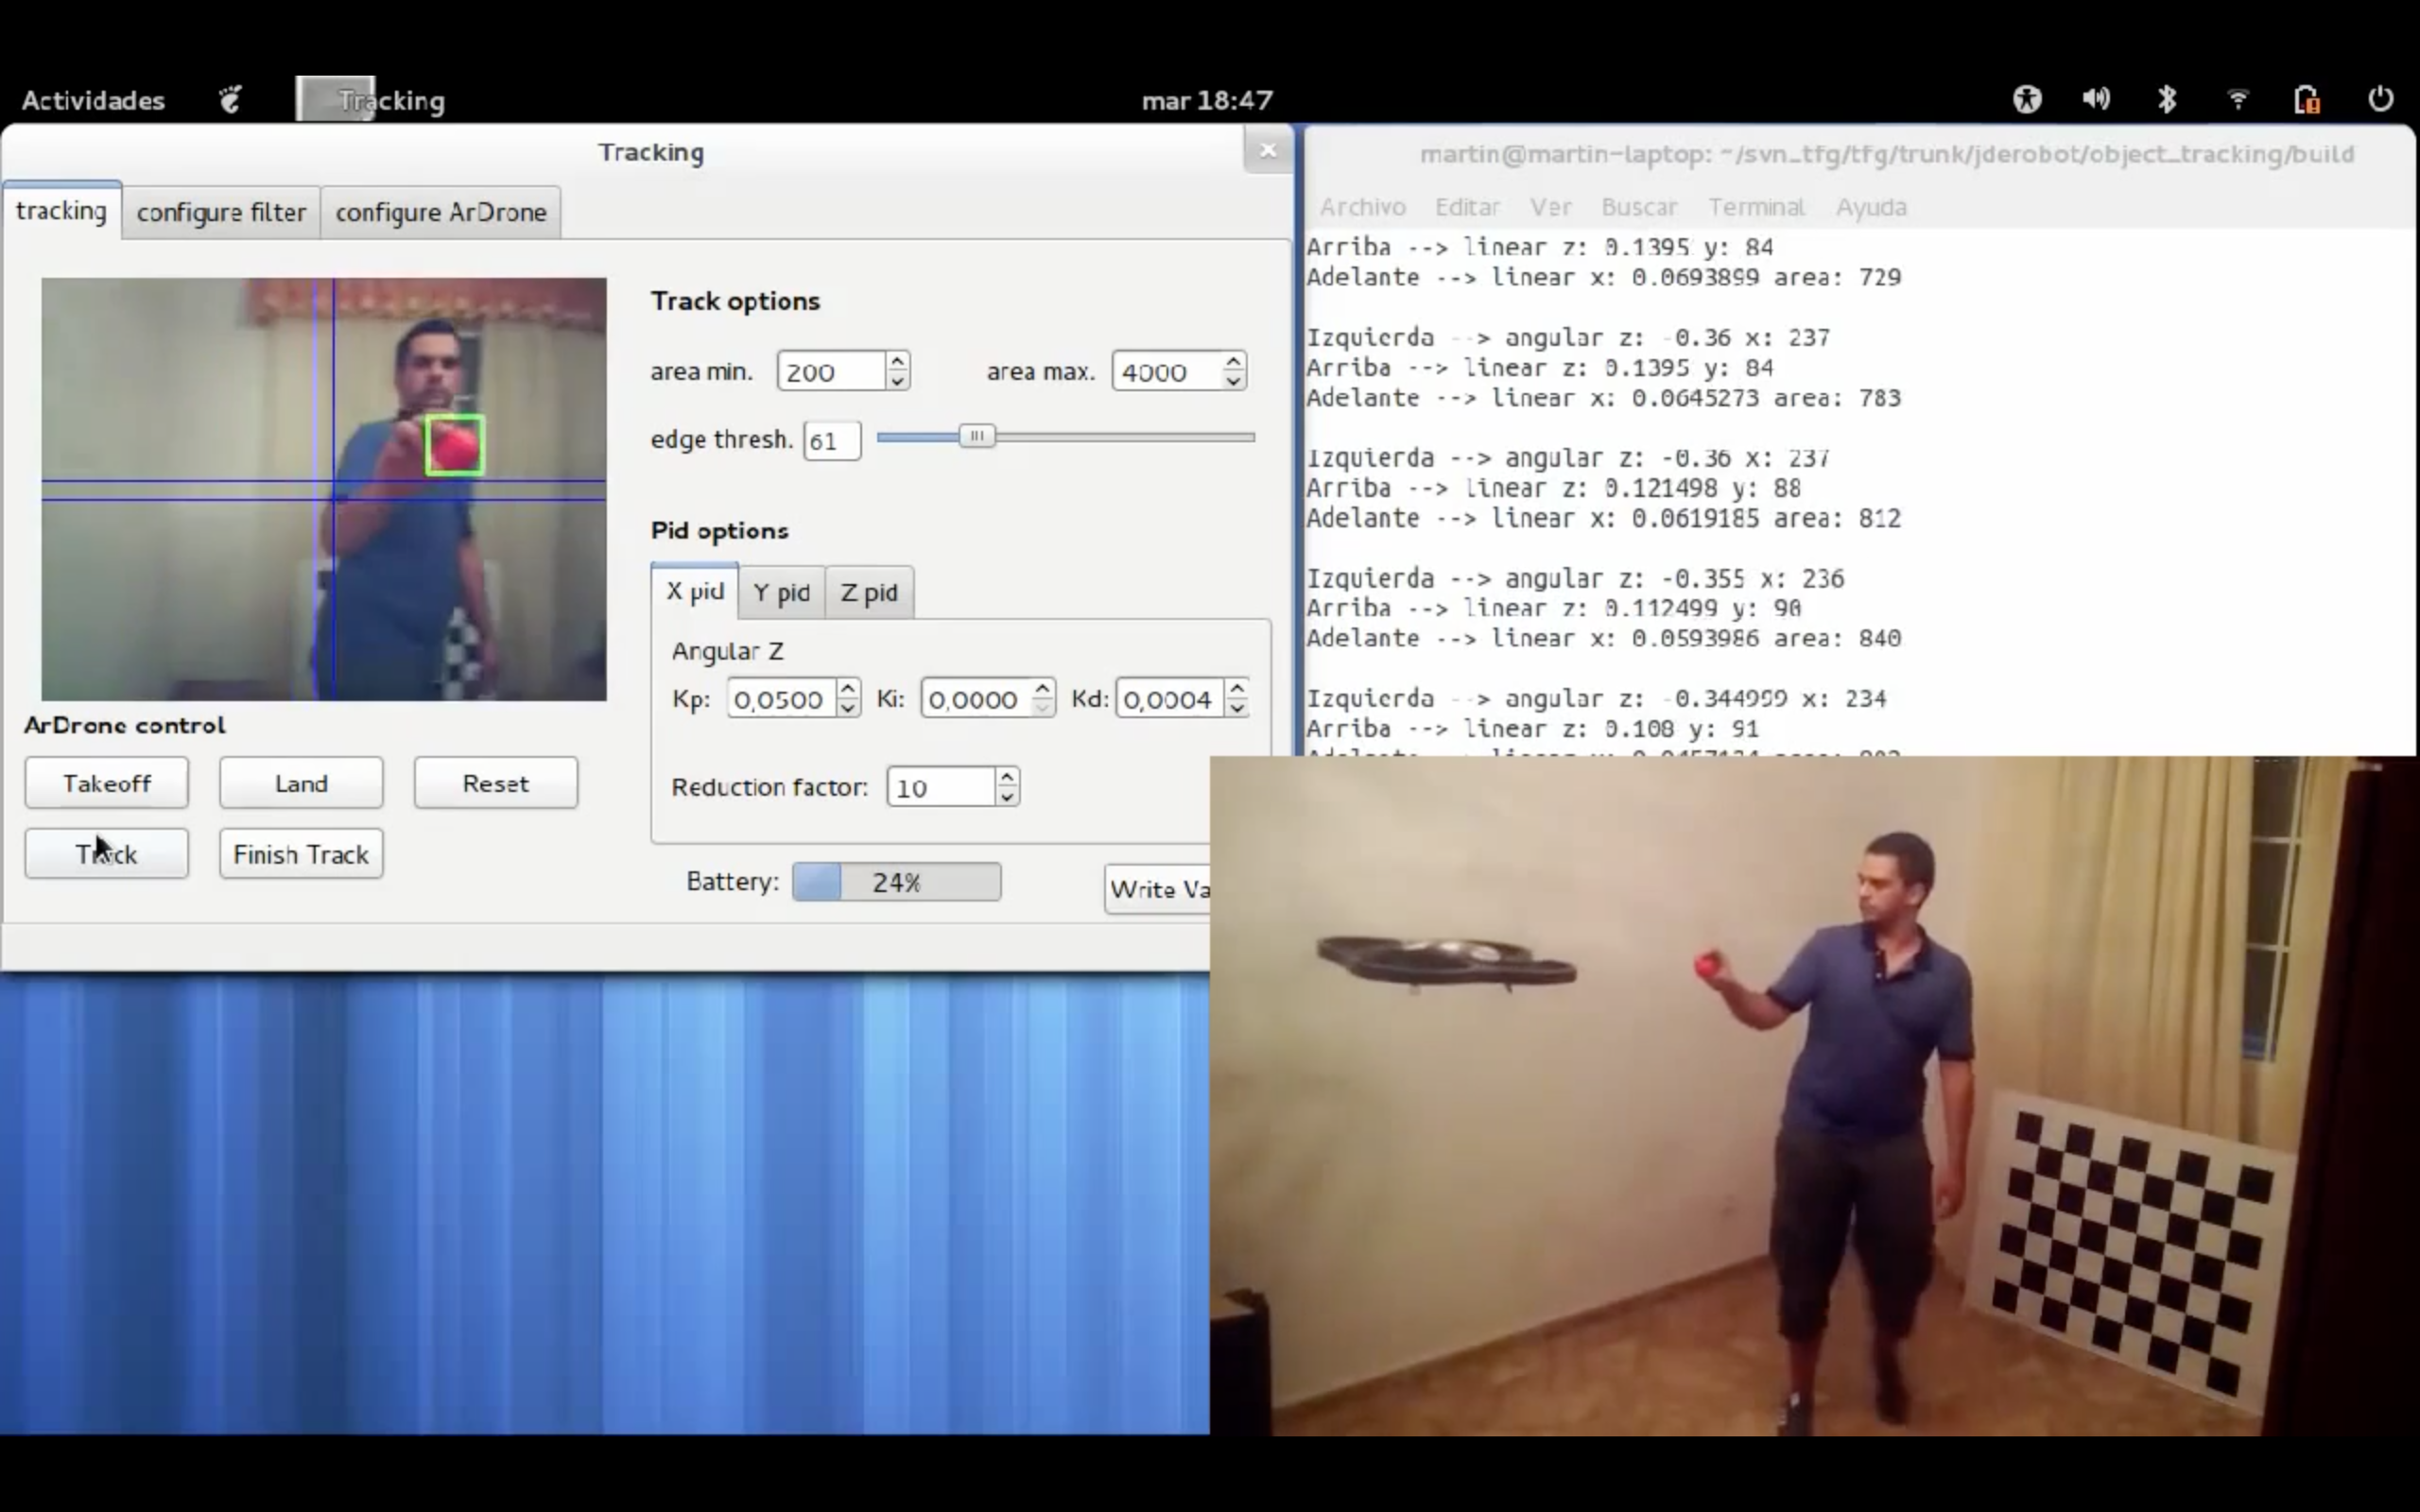
\includegraphics[width=0.9\textwidth]{ardroneserver_alberto}
\caption{Seguimiento horizontal usando ardrone\_server.}
\label{fig:ardroneserveralberto}
\end{figure}

\subsection{Surveillance 4.0}

Surveillance 4.0\footnote{\url{http://jderobot.org/D. castellanob-pfc}}\cite{surveillance4.0} es un ejemplo de conexión web con sensores y actuadores, desarrollado por Daniel Castellano como su Proyecto Fin de Carrera. Esta aplicación contaba con varios sensores de distinto tipo (humedad, temperatura, gas, etc) que se conectaban inalámbricamente con un nodo central situado en una Raspberry Pi. La conexión inalámbrica se hacía mediante transmisores Zigbee con un protocolo propio llamado WHAP. El nodo central recibía los datos de los sensores y los mostraba mediante un servidor web que corría en la misma máquina. La aplicación web se desarrolló en Python usando el entorno de desarrollo web Django. En Surveillance 4.0, los valores de los sensores se guardaban en una base de datos que la aplicación web consultaba cuando era necesario. Además, esta versión incluía un streaming de vídeo utilizando el software de código abierto M-JPEG Streamer. En la figura \ref{fig:surveillance4} se puede ver la aplicación.\\


\subsection{Surveillance 5.1}

Otro ejemplo de conexión web con sensores y actuadores es Surveillance 5.1\footnote{\url{http://jderobot.org/Aerobeat-colab}}\cite{surveillance5.1} desarrollado por Edgar Barrero como su Trabajo Fin de Grado. Esta aplicación obtenía un flujo de imágenes de una cámara web, un flujo de imágenes de profundidad de un sensor Kinect, además de datos de un sensor de humedad y de interaccionar con un actuador. La aplicación web se desarrolló en Ruby sobre Rails. En Surveillance 5.1, el servidor web se conectaba a los componente de JdeRobot mediante sus interfaces ICE. La aplicación web refrescaba estos datos mediante peticiones AJAX.  En la figura \ref{fig:surveillance5} se puede ver la aplicación.\\


\begin{figure}[h!]
\centering
  \begin{subfigure}[]{110mm}
    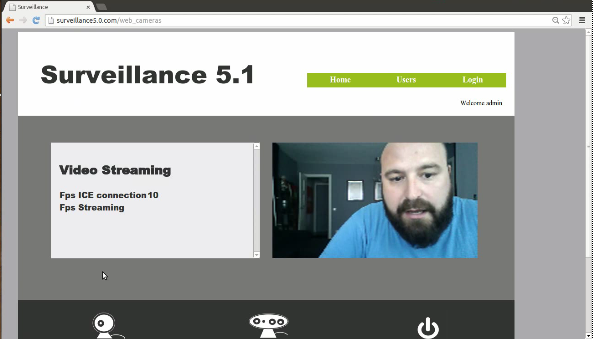
\includegraphics[width=110mm]{surveillance5}
  \end{subfigure}
  \hspace{5pt}
  \begin{subfigure}[]{110mm}
    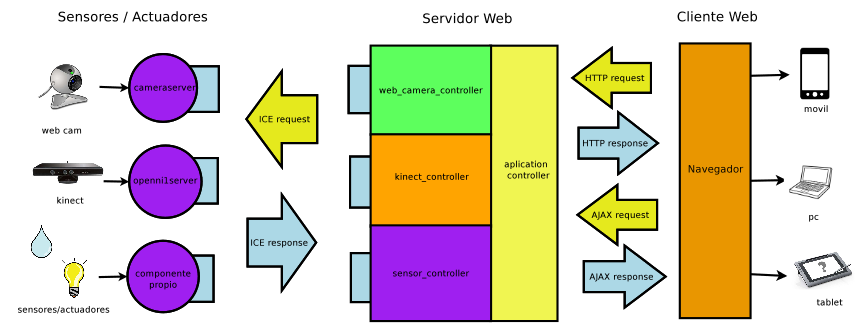
\includegraphics[width=110mm]{esquema_s5}
  \end{subfigure}
  \caption{interfaz (a) y arquitectura (b).}\label{fig:surveillance5}
\end{figure}


\subsection{Teleoperadores y visores Web en JdeRobot}

Un ejemplo ya sin servidores web intermedios, directo entre sensores, robots y navegadores web es esta plataforma desarrollada por Aitor Martínez como su Trabajo Fin de Grado\footnote{\url{http://jderobot.org/Aitormf-tfg}}\cite{teleoperadoresyvisoresweb}. Está compuesta por cuatro clientes Web: CameraViewJS, RGBDViewerJS, KobukiViewerJS y UavViewerJS, los cuales son las versiones web de las herramientas homónimas desarrolladas por JdeRobot. Estas nuevas herramientas hablan directamente con los servidores desarrollados por JdeRobot para acceder a los sensores y robots, y como diferencia principal destacable no necesitan de servidores intermedios para funcionar, utilizando \emph{websockets} para establecer las conexiones necesarias.\\

\noindent Las funcionalidades de estos clientes web son: 

\begin{enumerate}

\item \emph{CameraViewJS:} Cliente web similar a la herramienta \texttt{CameraView} para visualizar imágenes procedentes del servidor \texttt{Cameraserver}. 

\item \emph{RGBDViewerJS:} Cliente web similar a la herramienta RGBDViewer para visualizar datos de color y profundidad procedentes del servidor \texttt{Openni1Server}.
  
\item \emph{KobukiViewerJS:} Teleoperador para manejar y ver los datos de los sensores de los robots Kobuki y Pioneer del laboratorio de robótica de la URJC. Versión web de \texttt{KobukiViewer}
  
  
\item \emph{UavViewerJS:} Cliente web similar a la herramienta UavViewer para teleoperar drones tanto reales como simulados y ver los datos de sus sensores.


\end{enumerate}

\begin{figure}[h!]
\centering
\includegraphics[width=0.9\textwidth]{uavviewerjs_aitor}
\caption{Cliente web UavViewer.js}
\label{fig:introrobuavjs}
\end{figure}


En el proyecto que aquí se presenta se desarrolla una aplicación web capaz de teleoperar un cuadricóptero usando los servidores desarrollados por JdeRobot para conectarnos al drone, sus sensores y actuadores, y añadiendo la tecnología web de última generación \emph{WebRTC} para establecer la conexión entre el ordenador que se comunicará con el drone y el ordenador remoto. Desde el navegador se podrán ver los valores de los sensores y la cámara a bordo del drone, además como ya he mencionado, de teleoperarlo. Estas conexiones se realizarán sin el uso de servidor intermedio, usando tecnologías en tiempo real que se conectarán mediante \emph{WebSockets} de \emph{JavaScript}.\\


Una vez presentada la introducción y el contexto del proyecto en este capítulo, continuamos exponiendo los objetivos que nos hemos marcado. En el capítulo tres se habla sobre las infraestructuras software en las que nos hemos ayudado para el desarrollo. Posteriormente en el capítulo cuatro veremos cómo hemos conseguido cumplir los objetivos marcados, exponiendo en el capítulo cinco las pruebas y experimentos realizados. En el último capitulo presentaremos las conclusiones del proyecto.\\
